\section{Dynamic Responses to a Monetary Policy Shock in the Euro Area}\label{sec:results}
In this section, we discuss the responses to a restrictive monetary policy shock in the euro area. These responses are computed while explicitly conditioning on the US monetary policy stance. This exercise allows us to answer the question of how the monetary policy effect might change in the face of a divergent Fed policy. We therefore report and analyze impulse response functions (IRFs) based on our framework outlined in detail in \autoref{sec:framework}. 

Given our setup, we are able to trace how the transmission of ECB policy shocks varies with the \textit{entire} range of the Fed's stance. The transition function $g(z^\ast_t)$ delivers a distinct set of dynamic coefficients for every value of the Fed's stance, such that we have continuous mapping from the stance to the response of each variable. We therefore start with the continuum of responses in \autoref{fig:headline} for the one-week-ahead reaction of nominal government bond yields (top row), inflation swaps (middle row), and real yields (bottom row) at four selected maturities, plotting the response against the percentile of the Fed's stance. Reading the figure row-wise delivers our central result together with its economic decomposition.

\begin{figure}[!htpb]
\centering
\caption{One-week-ahead response of EA nominal yields, inflation swaps, and real yields to a restrictive ECB surprise, as a function of the Fed's monetary policy stance.}\label{fig:headline}
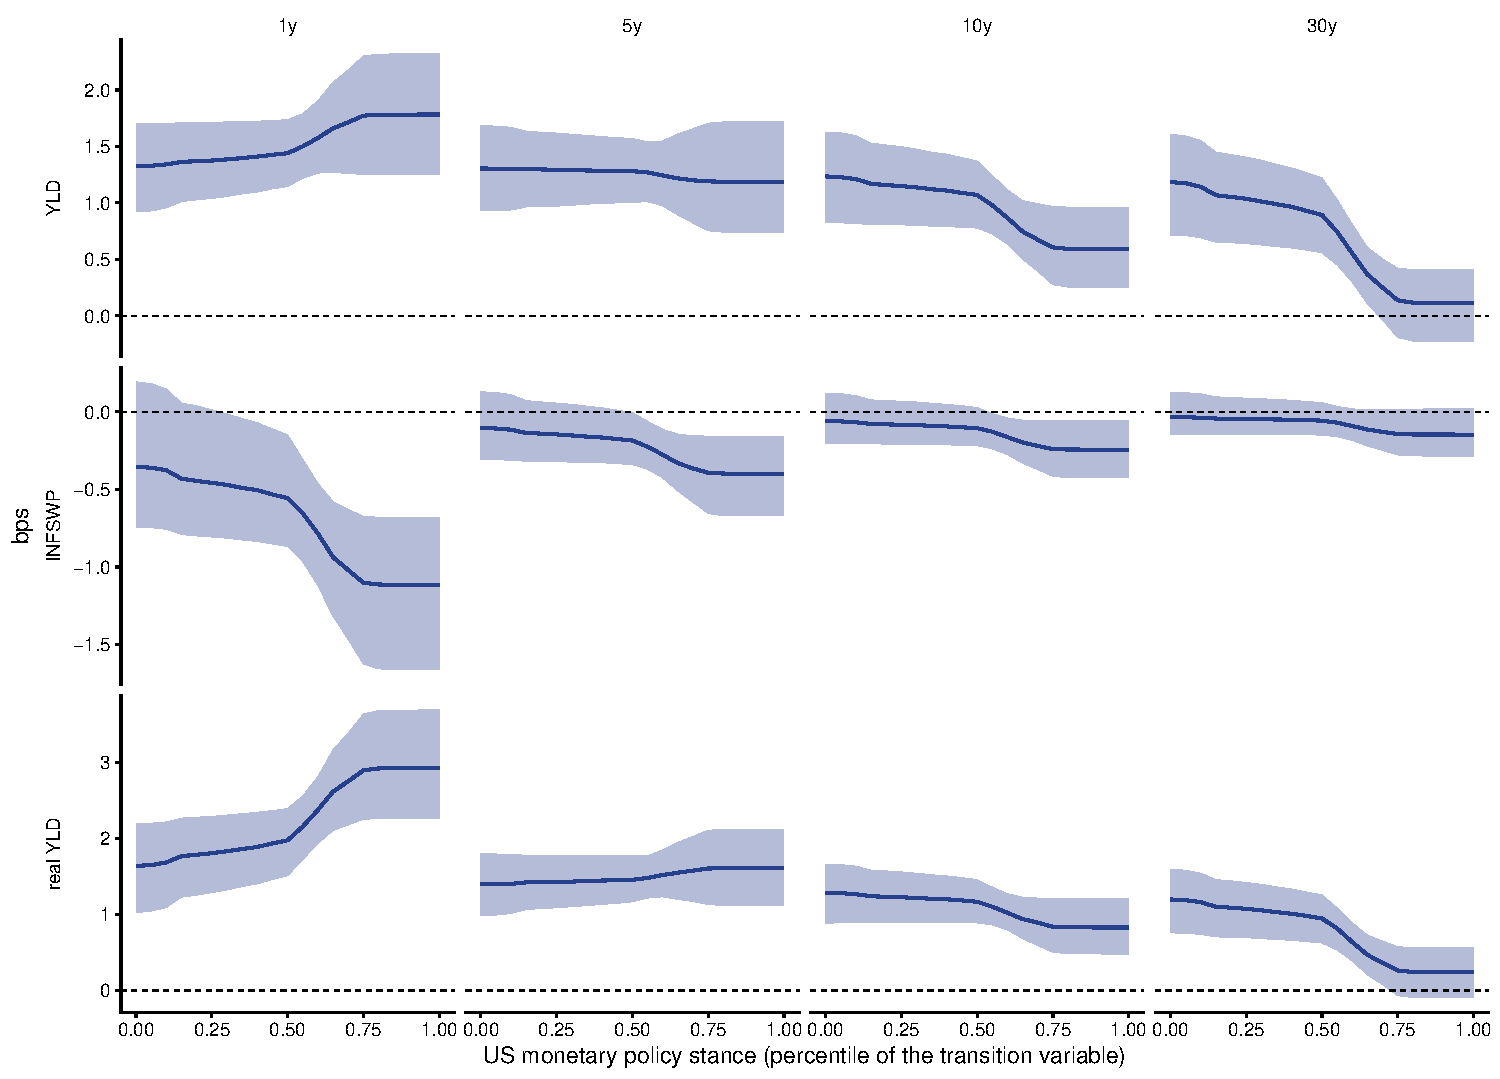
\includegraphics[width=\textwidth]{images_updated/rev/IRF_continuum_panel3.pdf}
\caption*{\footnotesize \textit{Notes:} Posterior median (solid) and $68\%$ credible set (shaded) of the one-week-ahead ($h=1$) response of the indicated variable to a one-standard-deviation restrictive ECB surprise, plotted against the percentile of the US monetary policy stance $z^\ast_t$ (0 = most accommodative, 1 = most restrictive). Rows: nominal government bond yields (YLD), inflation-linked swaps (INFSWP), and real yields (real YLD), where the real-yield response is computed draw-wise as the nominal minus the swap response. Columns: maturities of 1, 5, 10, and 30 years. Responses are in basis points.}
\end{figure}

%The central object of interest is how the transmission of an ECB surprise varies with the \textit{entire} range of the Fed's stance, not merely at two extremes. We therefore lead with the continuum of responses: because the transition function $g(z^\ast_t)$ delivers a distinct set of dynamic coefficients for every value of the Fed's stance, our model traces out a continuous mapping from the stance to the response of each variable. \autoref{fig:headline} presents this mapping for the one-week-ahead reaction of nominal government bond yields (top row), inflation swaps (middle row), and real yields (bottom row) at four selected maturities over the full 2005--2025 sample, plotting the response against the percentile of the Fed's stance. Reading the figure row-wise delivers the paper's central result together with its economic decomposition; note that, draw by draw, the nominal response equals the real response plus the response of inflation compensation.

The headline finding is that the Fed's stance does not shift the pass-through of ECB surprises up or down: it \textit{rotates} it. When the Fed is accommodative, a restrictive ECB surprise raises nominal yields by a similar amount along the whole curve, from $1.3$ basis points at one year to $1.2$ at thirty. When the Fed is restrictive (ninety-fifth percentile), the same surprise raises the one-year yield by more ($1.8$ basis points) but the reaction then falls monotonically with maturity, to $1.2$ basis points at five years, $0.6$ at ten, and $0.1$ at thirty, where it can no longer be distinguished from zero. The two profiles cross between three and five years. Thus, the state dependence is absent at the short end, where the accommodative response falls short of the restrictive one and becomes both sizeable and well determined at the long end. The state dependence of ECB transmission is thus a phenomenon of the \textit{long} end of the curve.

This maturity pattern is thus not uniform. Short-dated yields are governed by the expected path of the ECB's own policy rate, which responds to a domestic surprise in much the same way whatever the external environment. Long-dated yields, by contrast, embed a substantial term premium, and it is this component that is compressed and rendered more sensitive to policy news when US policy is accommodative and global risk appetite is high \citep{miranda2020us}. When the Fed itself is tight, that amplification is absent and an ECB tightening no longer moves the long end at all.

The middle and bottom rows show that the fading of the \textit{nominal} response at long maturities does not mean that policy stops working. At the short end, in particular, it conceals a pronounced change in composition. A contractionary surprise lowers inflation compensation whatever the Fed is doing, but it does so far more forcefully when the Fed is restrictive. Under an accommodative Fed the swap response is small and imprecisely estimated, $-0.4$ basis points at one year and no more than $0.2$ from three years out, so the nominal reaction is almost entirely a real-rate reaction. Under a restrictive Fed inflation compensation falls significantly out to fifteen years, and strongly at the short end. The difference between the two regimes is itself significant at one and three years but not beyond, so the inflation-expectations channel of the state dependence is a short-end phenomenon. Interestingly it is the mirror image of the nominal result, which is a long-end one. The bottom row shows the consequence. The one-year real yield rises by $2.9$ basis points under a restrictive Fed, against $1.7$ under an accommodative one. An ECB tightening delivered while the Fed is tight therefore tightens real short-term financing conditions appreciably more than the modest difference in the nominal short-end response suggests, and it does so by lowering expected inflation rather than by raising the nominal rate. At long maturities the real response fades along with the nominal one, leaving the term-premium interpretation intact.\footnote{Most of the identification that makes this continuum so sharp, comes from the pronounced Fed-ECB divergence of 2022-2024. It supplies exactly the restrictive-Fed observations that were scarce before the pandemic. } A heatmap over the \textit{full} term structure and all stance percentiles is provided in \autoref{fig:continuumheat} in Appendix~\ref{app:A}.



%The remainder of this section proceeds as follows. We first discuss the dynamic responses of government bond yields; the corresponding dynamic responses of inflation swaps and real yields, whose impact behavior is already summarized by \autoref{fig:headline}, are delegated to Appendix~\ref{app:A}, as are the responses of the remaining macro-financial variables --- the exchange rate, stock prices, and systemic stress. \autoref{sec:extended} discusses what the 2022--2024 divergence episode contributes to identification. All results are estimated on the full 2005--2025 sample --- the extended inflation swap data now cover the entire sample period --- and are based on the updated data vintage described in \autoref{sec:Data}.



\subsection{Dynamic responses of the government bond yield curve}

We now move to the full impulse horizon and fix two reference points along the continuum. The first sets the threshold variable $z_t^\ast$ to its $95\%$ percentile, a strongly \textit{tight} Fed in red; the second sets it to the $5\%$ percentile, a strongly \textit{loose} Fed in blue. Comparing these two extremes isolates the largest possible difference in transmission but it also yields the noisiest contrasts. We therefore treat the two-extreme comparison as illustrative and rely on the full continuum in \autoref{fig:headline} for inference. In the figures that follow, the top panel shows the responses under the two reference stances over the impulse horizon and the bottom panel their difference; the corresponding impact responses across the continuum of stances are those already reported in \autoref{fig:headline}. Recall that the model is specified in weekly \textit{first differences}, so the panels show weekly \textit{changes} in yields. 

\begin{figure}[!htpb]
\caption{Impulse responses of a restrictive EA monetary policy shock for selected government bond yields. \label{fig:IRFylds}}
\begin{minipage}{\textwidth}
\centering
a) Responses for two scenarios of US monetary policy
\end{minipage}
\begin{minipage}{\textwidth}
\centering
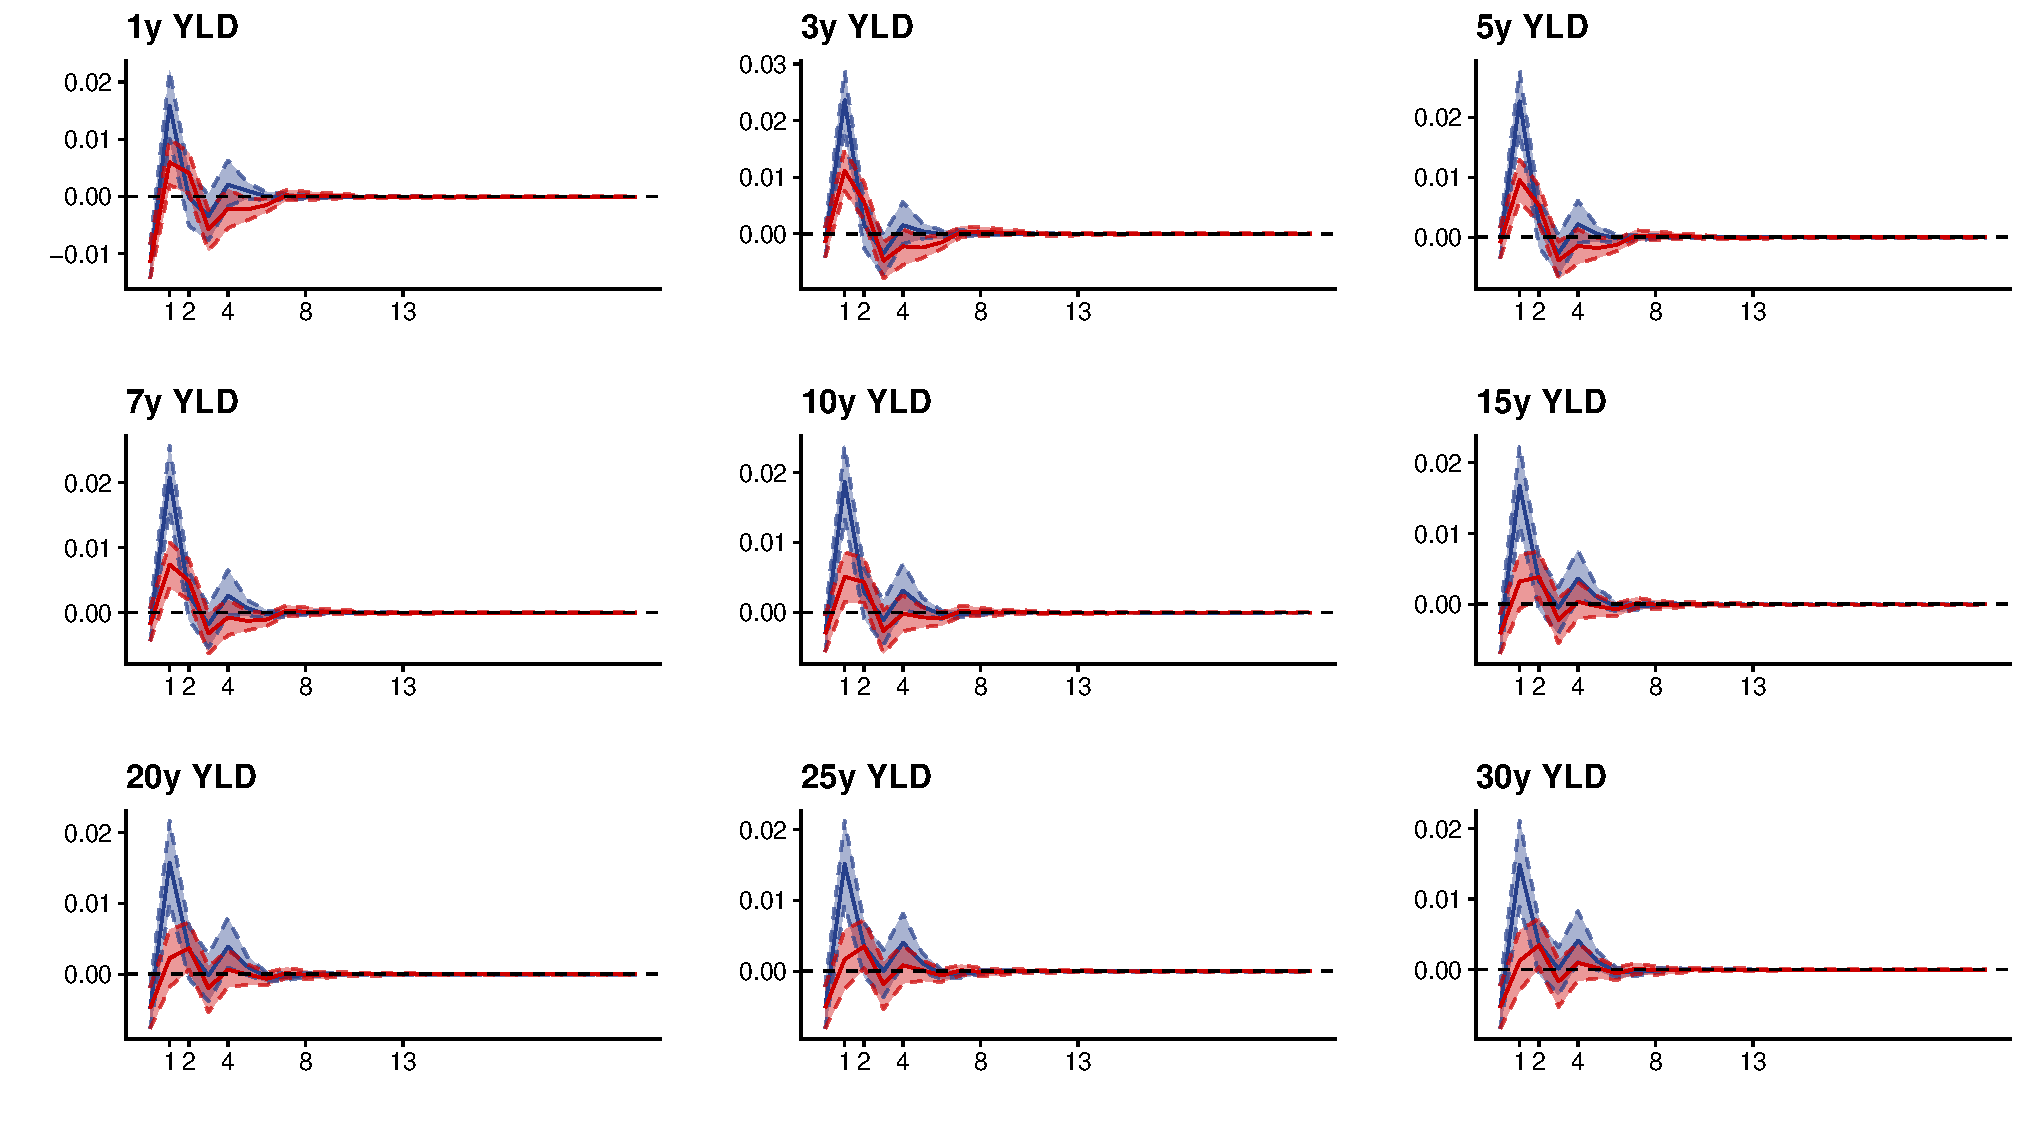
\includegraphics[width=0.85\textwidth]{images_updated/DIFF_EA_Motto/IRF_YLDS_LH_SLCT.pdf}
\end{minipage}
\begin{minipage}{\textwidth}
\centering
b) Difference in responses
\end{minipage}
\begin{minipage}{1\textwidth}
\centering
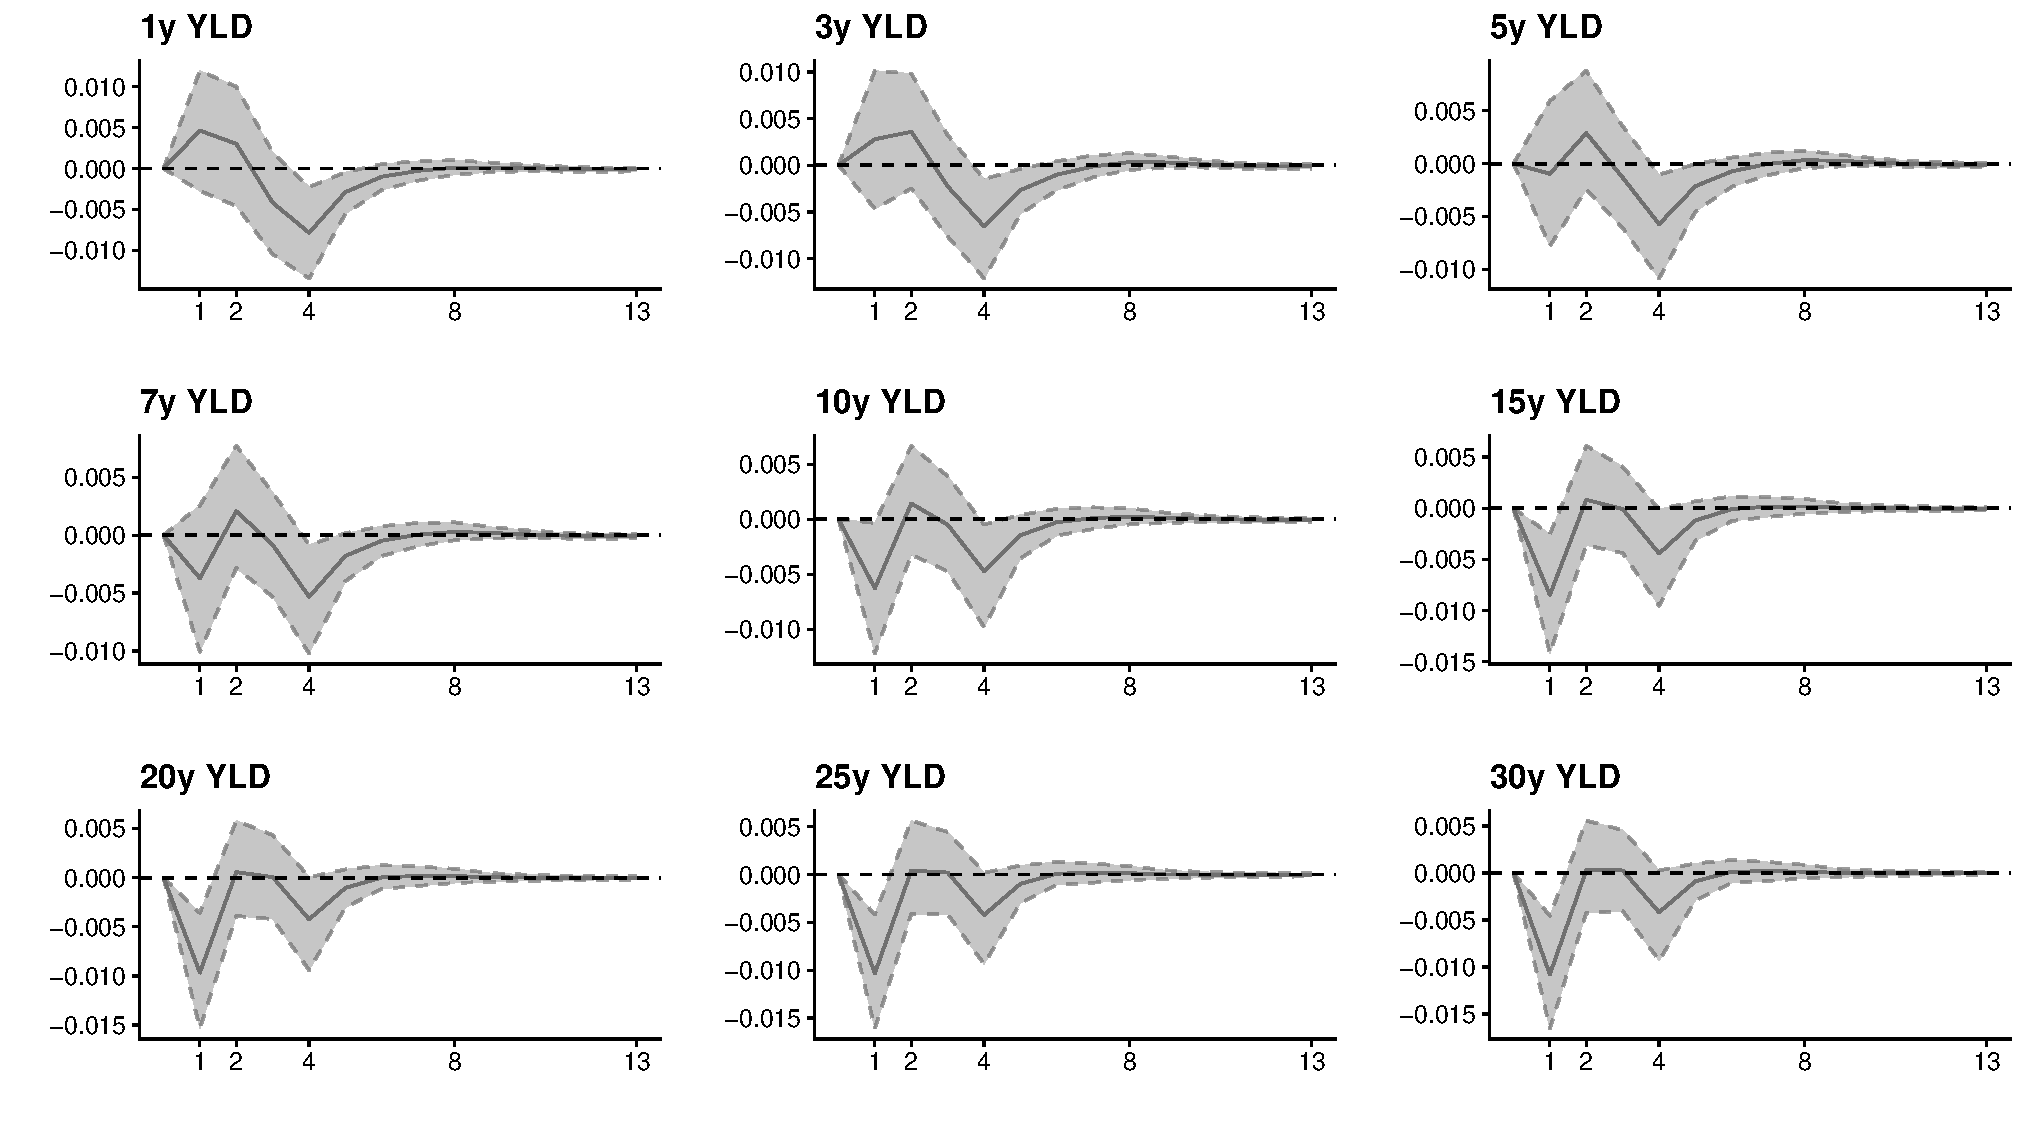
\includegraphics[width=0.85\textwidth]{images_updated/DIFF_EA_Motto/IRF_YLDS_D_SLCT.pdf}
\end{minipage}
\caption*{\footnotesize \textit{Notes:} Panel (a) plots the responses to a contractionary monetary policy shock in the EA conditional on two scenarios: A restrictive US monetary policy stance (95$\%$ percentile of the threshold, colored in red) and an expansionary US monetary policy stance (5$\%$ percentile of the threshold, colored in blue). Panel (b) plots the differences between the two US regimes (restrictive minus expansionary stance). In both panels, the horizontal axis indicates the weeks following the shock. The shaded areas denote the $68\%$ posterior credible set and the solid line denotes the posterior median. Responses are weekly changes in percentage points.}
\end{figure}


Inspecting \autoref{fig:IRFylds}, we find that in both regimes, government bond yields rise on impact after a restrictive monetary policy shock, and in both the reaction is concentrated in the first week and has died out within roughly six weeks. What differs across regimes is the maturity profile. Comparing the blue and red lines in panel (a), the two regimes are statistically indistinguishable at the short end. However, the gap then opens up, and changes sign, as maturity increases. Panel (b) shows this difference to be significantly negative for every maturity from ten years upwards, and insignificant at one, three, and five years. This clean monotone pattern matches the continuum in \autoref{fig:headline} and, hence, the term-premium mechanism that motivates it.  More generally, the two-extreme comparison is illustrative as it contrasts two tail stances. Thus it discards the intermediate observations that carry most of the identifying information, which is why the credible sets in panel (b) are wide beyond the impact week. 



\subsection{Exchange rate, equities, and systemic stress}

Our model also includes the euro--dollar exchange rate, stock market returns, and the CISS. \autoref{fig:IRFOTHER} reports their responses under the two reference stances of the Fed, together with the difference between the two. The Fed's stance matters here too, and in opposite directions for the two asset classes. The euro appreciates by $0.13$ percent one week after a restrictive surprise when the Fed is accommodative, and essentially not at all when the Fed is restrictive, which is what the mechanism of \autoref{fig:headline} implies: a loose Fed leaves more room for an ECB surprise to move the transatlantic differential. The difference between the regimes is not itself statistically significant, however, so we read it as suggestive only. Equities fall by about $0.4$ percent under either stance. The regimes diverge thereafter: one week out the decline has largely reversed under an accommodative Fed, to $0.06$ percent, but persists at $0.15$ percent under a restrictive one, and this difference is significant. That ordering follows the real-rate result rather than the nominal one: an ECB tightening delivered into a tight Fed raises the short real rate by considerably more, and it is the real discount rate that equities price. The systemic stress indicator behaves differently. The CISS rises after a restrictive surprise in both regimes, but by more, and more persistently, when the Fed is \textit{restrictive}. The sign is economically sensible: a domestic tightening that arrives on top of an already tight global financial environment adds to funding stress, whereas the same surprise under an accommodative Fed is cushioned by ample global liquidity. Note also that, since we use only triple-A rated sovereign bonds, safe-haven motives within the euro area play little role in these results.

\begin{figure}[!htpb]
\caption{Impulse responses of a restrictive EA monetary policy shock for other quantities.\label{fig:IRFOTHER}}
\begin{minipage}{\textwidth}
\centering
a) Responses for two scenarios of US monetary policy
\end{minipage}
\begin{minipage}{\textwidth}
\centering
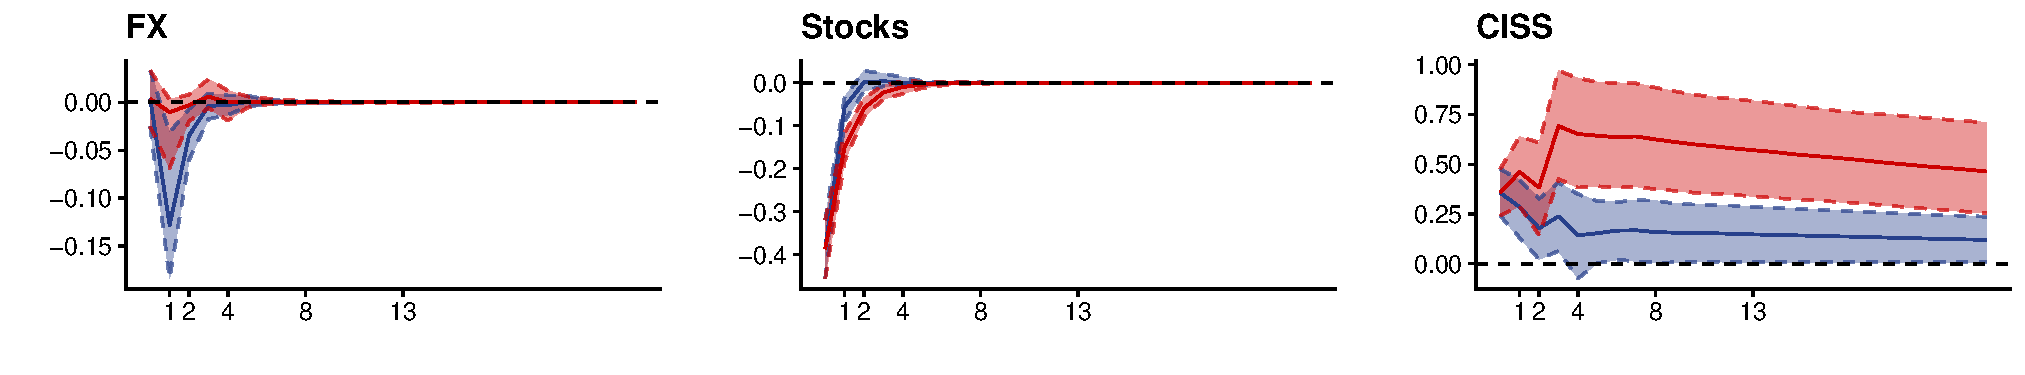
\includegraphics[width= \textwidth]{images_updated/DIFF_EA_Motto/IRFOTHERS_LH.pdf}
\end{minipage}
\begin{minipage}{\textwidth}
\centering
b) Difference in responses
\end{minipage}
\begin{minipage}{1\textwidth}
\centering
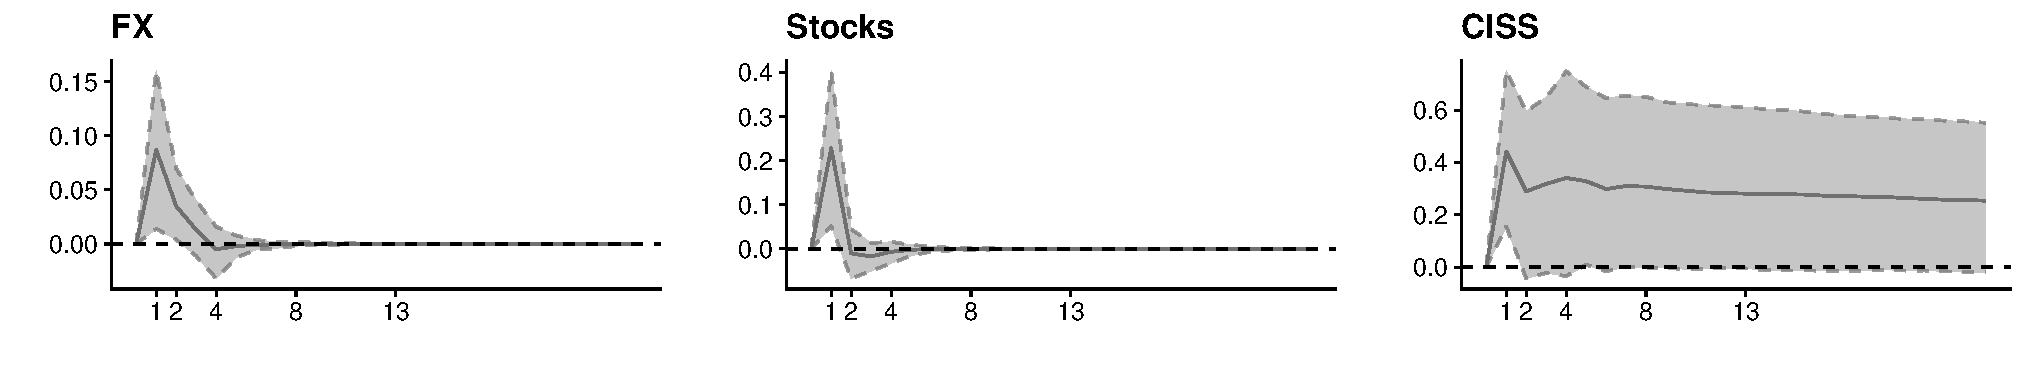
\includegraphics[width= \textwidth]{images_updated/DIFF_EA_Motto/IRFOTHERS_D.pdf}
\end{minipage}
\caption*{\footnotesize \textit{Notes:} Panel (a) plots the responses to a contractionary monetary policy shock in the EA conditional on two scenarios: A restrictive US monetary policy stance (95$\%$ percentile of the threshold, colored in red) and an expansionary US monetary policy stance (5$\%$ percentile of the threshold, colored in blue). Panel (b) plots the differences between the two US regimes (restrictive minus expansionary stance). In both panels, the horizontal axis indicates the weeks following the shock. The shaded areas denote the $68\%$ posterior credible set and the solid line denotes the posterior median. FX denotes the Euro per one US-dollar (i.e., a decrease denotes an appreciation of the Euro), Stocks the Euro Stoxx 50 index, and CISS the Composite Index of Systemic Stress.}
\end{figure}


% {\color{red}
% \subsection{Controlling for global factors}\label{sec:global}
% A natural concern with our identification strategy is that the Fed's stance may partly reflect common global conditions rather than US monetary policy per se. During a synchronized global inflation cycle, for instance, the Fed may be tight at the same time as commodity prices, the dollar, and global risk aversion move, and it could be these global forces, rather than US policy, that alter the transmission of ECB surprises. We address this concern in two complementary ways.

% First, we augment the vector $\bm y_t$ with three global variables that are available at daily frequency and span the main dimensions of the global cycle: the Brent oil price (in percentage changes), the broad nominal US dollar index (in percentage changes), and the VIX as a proxy for global risk aversion. These variables enter both regimes and are allowed to react to, and feed back into, all EA quantities. \autoref{fig:IRFglobal} shows the yield curve responses from this extended model. They are remarkably close to the baseline: yield reactions to a restrictive ECB surprise remain significantly stronger under an accommodative Fed, with the one-week-ahead difference at short maturities significant at the $68\%$ level, and the maturity profile of the differences is unchanged. The global variables themselves react little to the ECB surprise, consistent with the euro area being small relative to global financial markets.

% Second, we purge the stance measure itself of the global cycle. We regress $z_t^{\ast}$ on year-on-year oil price growth, year-on-year growth of the broad dollar index, and the level of the VIX, and use the residual --- the component of the Fed's stance that is orthogonal to these global factors --- as the transition variable. The resulting regime allocation is nearly identical to the baseline (the correlation of the posterior mean of $S_t$ across the two specifications is $0.95$), confirming that our stance measure is not simply a repackaged global cycle. The impulse responses retain the same pattern, although the differences between regimes lose some statistical precision, which is expected given that the purging step removes variation that is informative about the stance itself. Taken together, these exercises indicate that the state dependence we document is attributable to the US policy stance and not to omitted global variables, although we acknowledge that no reduced-form exercise can fully isolate US monetary policy from the global conditions to which it responds.

% \begin{figure}[!htpb]
% \caption{\rev{Impulse responses of government bond yields in the model with global variables.} \label{fig:IRFglobal}}
% \begin{minipage}{\textwidth}
% \centering
% a) Responses for two scenarios of US monetary policy
% \end{minipage}
% \begin{minipage}{\textwidth}
% \centering
% 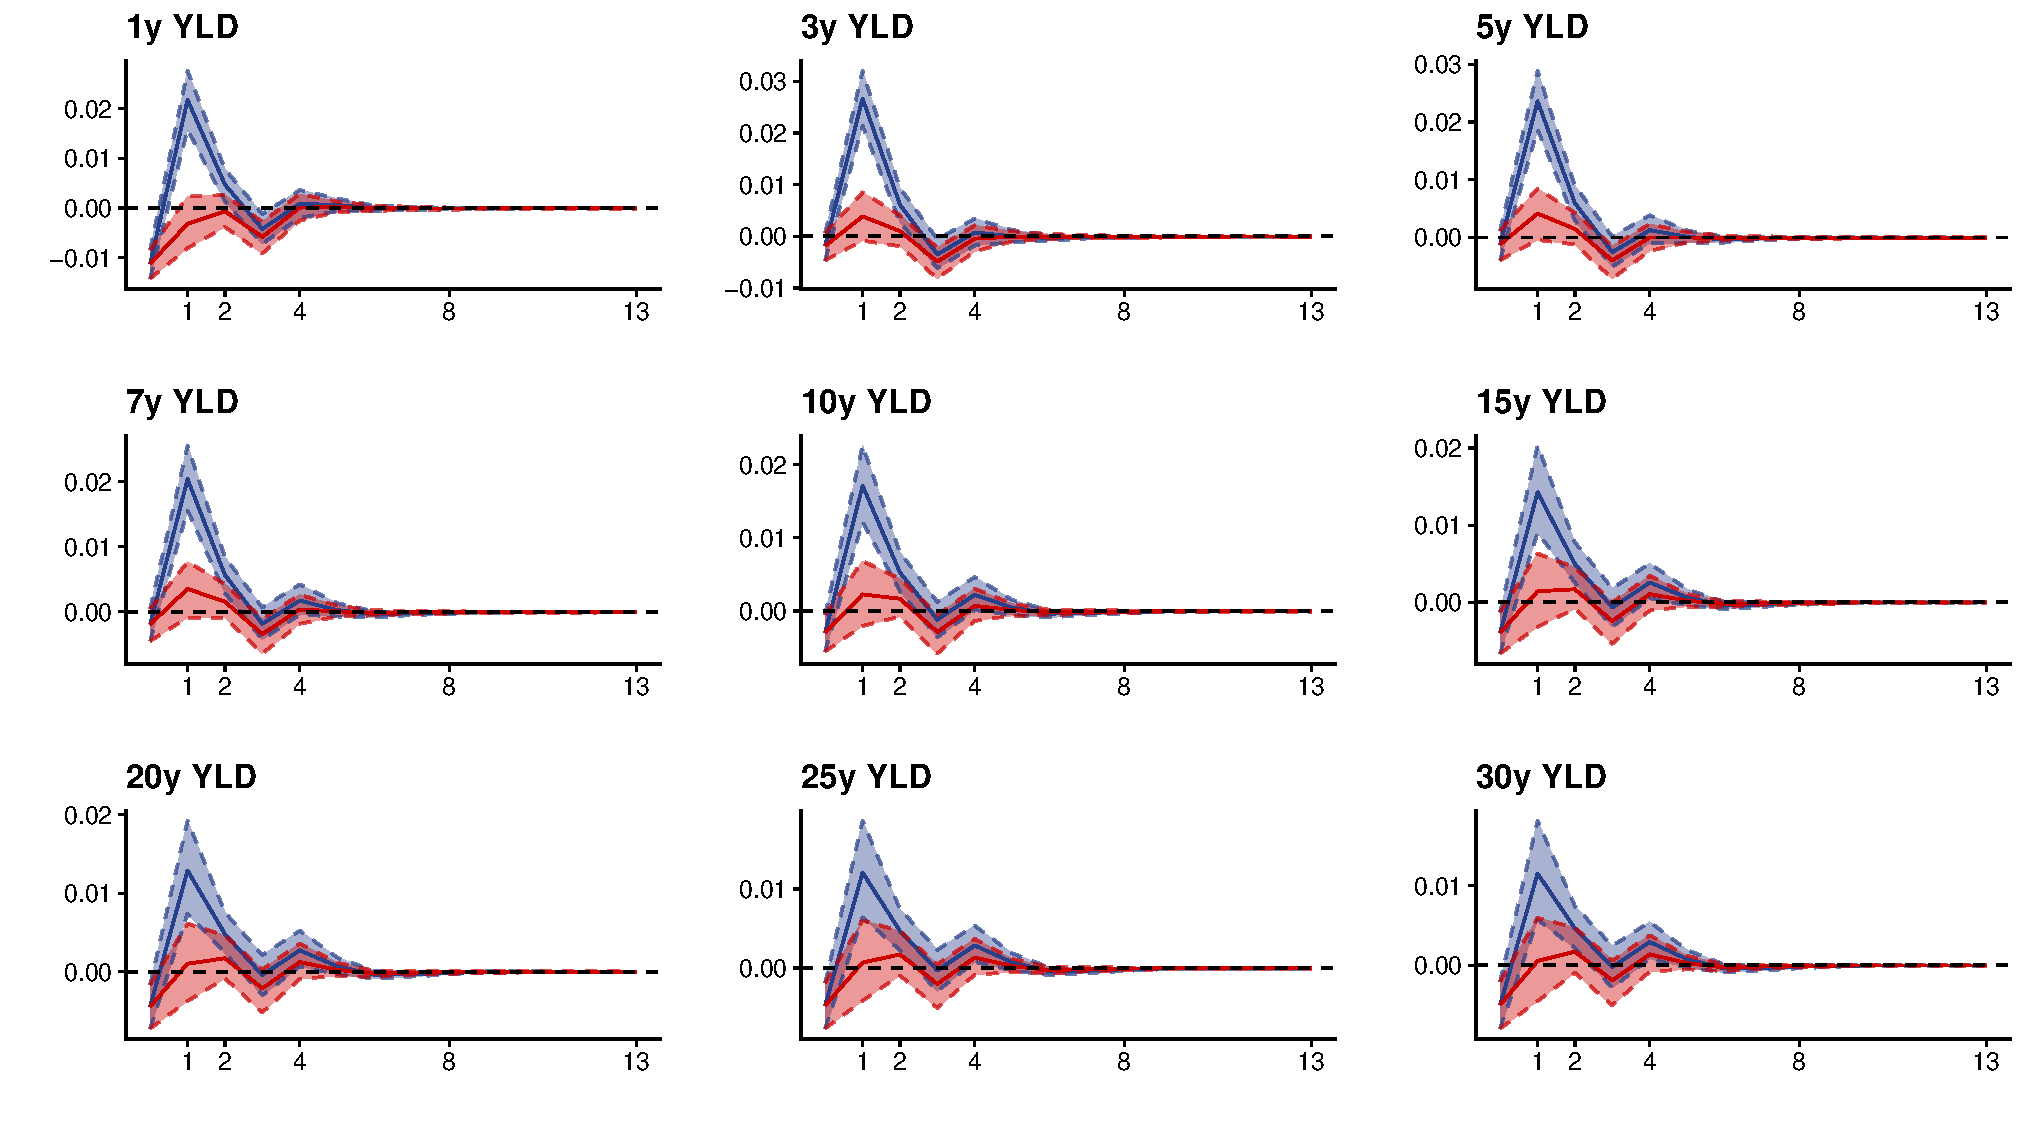
\includegraphics[width=0.7\textwidth]{images/rev/IRF_YLDS_GLOB19_LH_SLCT.pdf}
% \end{minipage}
% \begin{minipage}{\textwidth}
% \centering
% b) Difference in responses
% \end{minipage}
% \begin{minipage}{1\textwidth}
% \centering
% 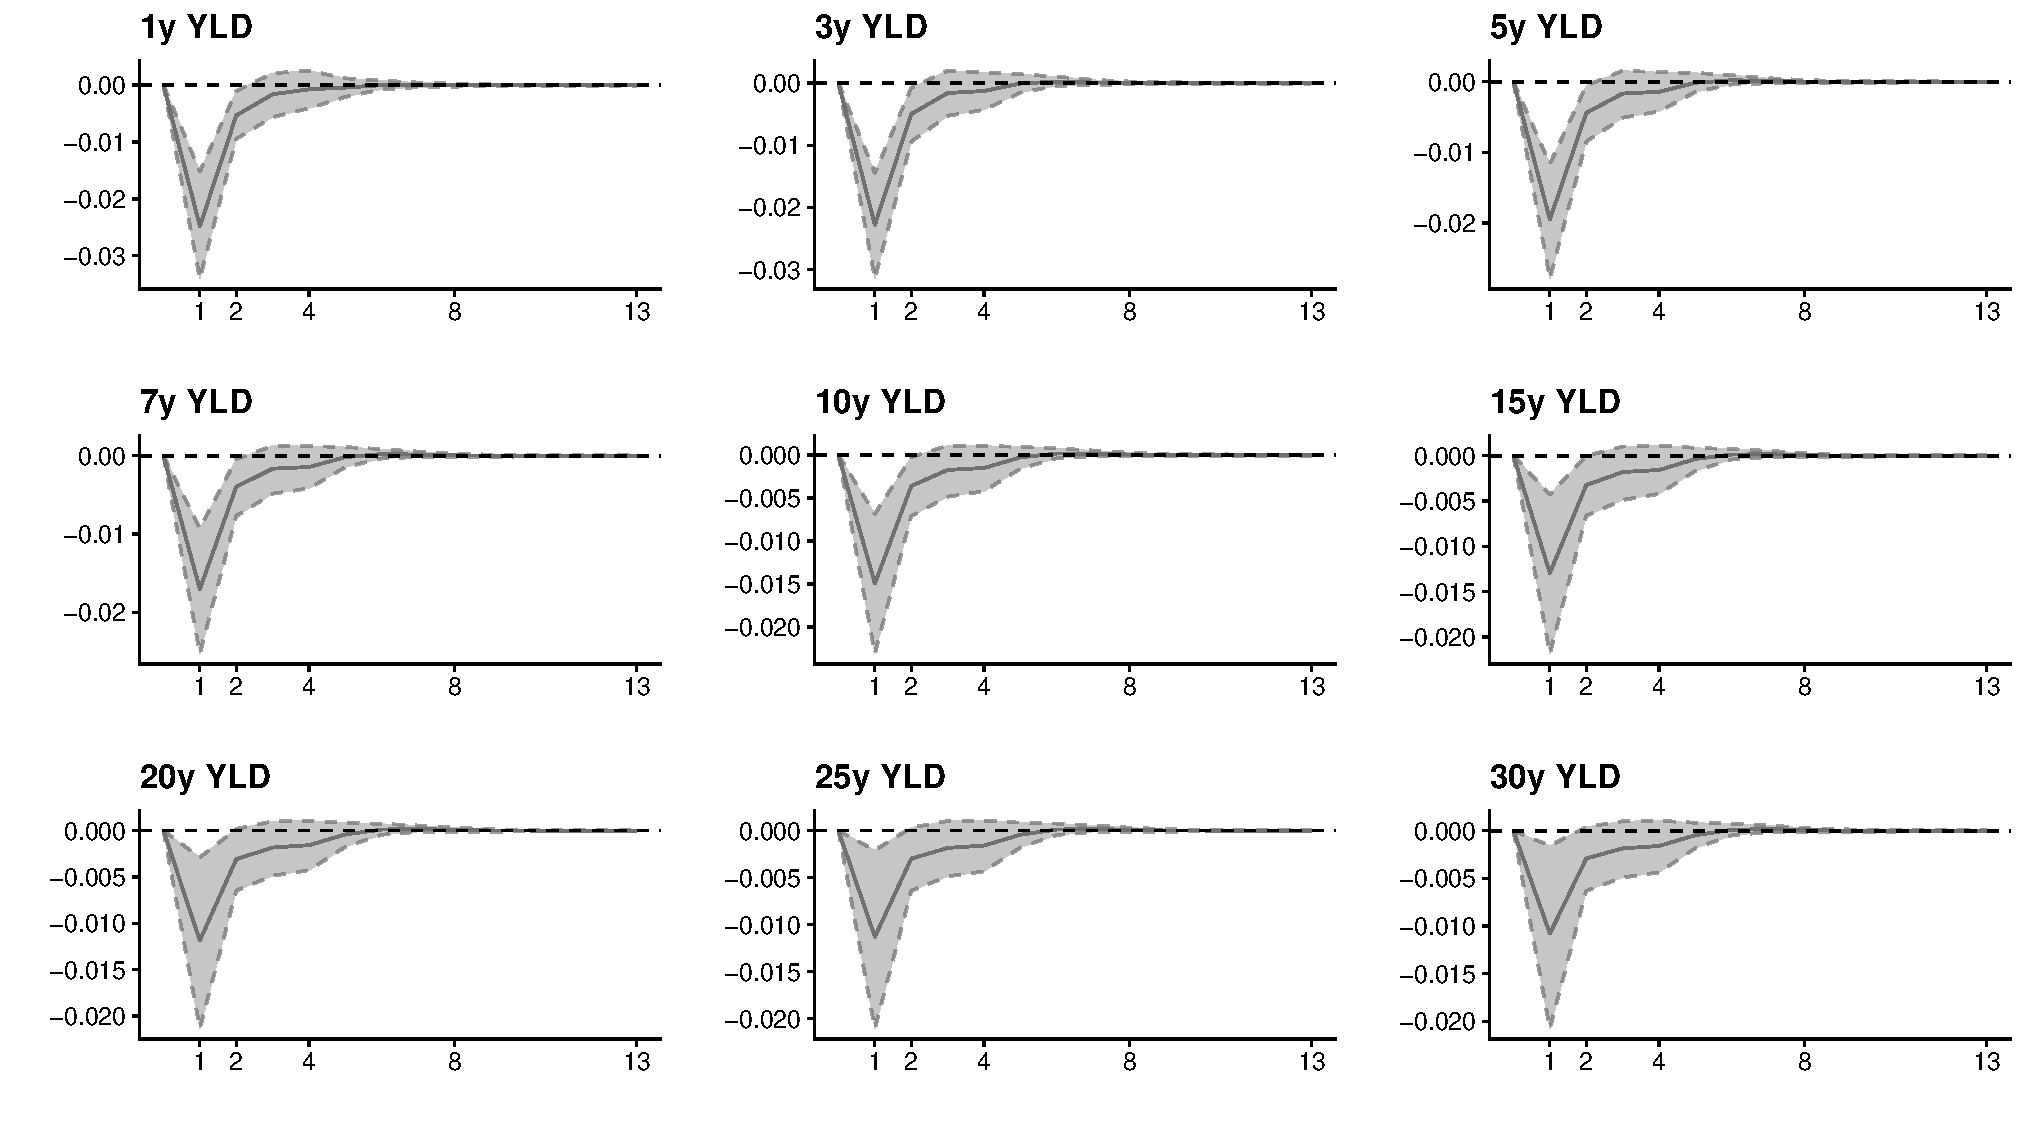
\includegraphics[width=0.7\textwidth]{images/rev/IRF_YLDS_GLOB19_D_SLCT.pdf}
% \end{minipage}
% \caption*{\footnotesize \textit{Notes:} \rev{Responses to a contractionary EA monetary policy shock in the specification that augments $\bm y_t$ with the Brent oil price, the broad US dollar index, and the VIX, estimated over the full 2005--2026 sample. Panel (a) conditions on a restrictive (95\% percentile, red) and an expansionary (5\% percentile, blue) US stance; panel (b) shows the difference (restrictive minus expansionary). Shaded areas denote the 68\% posterior credible set.}}
% \end{figure}




\subsection{Robustness}\label{sec:results_rob}
The rotation documented above rests on two constructed inputs and two  parameters. The stance measure decides \textit{when} the Fed is restrictive, thus impacting the state allocation, while the monetary policy surprise measure decides \textit{what} an ECB policy shock is, impacting the dynamic responses. Finally, the transition parameters $\mu$ and $\rho$ fix the location and sharpness of the boundary between regimes. For robustness checks, we vary each in turn, holding the others at baseline. Appendix~\ref{app:rob} collects the results with an overview of the specifications in \autoref{tab:robspecs}.

%Replacing the stance with the shadow short rate of \cite{krippner2016ems} relative to $r^{\ast}$ leaves the regime dating essentially untouched: the two posterior transition paths correlate at $0.95$, and both assign $41.0\%$ of weeks to the restrictive regime. Replacing the identification with the median-rotation shocks of \cite{jarocinski2020deconstructing} changes the impulse itself and is the more demanding test. Moving the neutral cut by a quarter and by half a percentage point of the stance reclassifies up to $148$ of $1{,}090$ weeks and shifts the restrictive share from $34.8\%$ to $54.6\%$; the sustained restrictive phase from mid-2022 to the end of the sample stays restrictive under every cut. Centering the steepness prior at seven rather than four leaves the responses virtually unchanged (correlation of posterior medians $0.998$, maximum deviation $0.17$ basis points).

The results are robust to alternative measures of the policy stance, identification schemes, regime thresholds, and prior specifications. Although these choices affect the classification of some weeks and, in the case of alternative shocks, the estimated impulse itself, the main pattern of a sustained restrictive US monetary policy stance since mid-2022 and the resulting impulse responses remains unchanged.

Across all eight specifications, the rotation is preserved. Short-maturity responses are significantly positive across the entire stance distribution after a restrictive EA MP shock, whereas long-maturity responses become insignificant under sufficiently restrictive US monetary policy. The loose-minus-tight differential is negative at short maturities, close to zero in the belly of the curve, and positive and increasing from ten years onward. Thus, the sign and maturity profile of the state dependence are robust to alternative measurements, calibrations, and identification schemes.


%Across all eight specifications the rotation is present without exception. The response at short maturities is significantly positive at every point of the stance distribution, while at thirty years it ceases to be so somewhere between the fifty-fifth and the seventieth percentile in every one of the eight. The gap between the regimes is negative at one year, indistinguishable from zero in the belly of the curve, and positive and increasing in maturity from ten years out, in every specification. The sign and the maturity profile of the state dependence are therefore not artifacts of measurement or calibration: the posterior probability of a positive loose-minus-tight gap at thirty years is at least $0.88$ in seven of the eight specifications and $0.81$ in the remaining one, which replaces our composite surprise with the alternative identification.

%%% [superseded by the following paragraph -- commented out 2026-07-27] Its magnitude is more sensitive, and we are correspondingly careful with it. The thirty-year gap ranges from $0.48$ basis points under the alternative identification to $1.22$ under the widest regime definition. Most of that range is attributable to the identification of the surprise rather than to the calibration: across the four alternative cuts the gap varies only between $0.79$ and $1.22$ basis points, and lowering the cut widens it monotonically, since a lower cut confines the accommodative state to more deeply accommodative weeks. For the same reason we attach no interpretation to the shape of the accommodative-Fed profile in \autoref{fig:headline}, which tilts in either direction under modest changes in the cut: what is robust is the \textit{contrast} between the two states, not the shape of the response within either. We therefore read the evidence as establishing that euro area long-rate pass-through is weaker when the Fed is restrictive, and we report the size of that difference as a range rather than a point estimate.

The magnitude of the effect is more sensitive. At the thirty-year maturity, the loose-minus-tight gap ranges from $0.48$ to $1.22$ basis points, with most variation attributable to the identification of the policy surprise rather than to alternative regime definitions. We therefore refrain from interpreting the precise shape of responses within the accommodative state. The robust finding is instead the contrast across states: euro area long-rate pass-through is weaker when the Fed is restrictive. We consequently report the estimated difference as a range rather than a point estimate.


